\ifdefined\ispartofbook
\else
  % Preamble for "A Journey into Deep Learning"

% --- DOCUMENT CLASS & GEOMETRY ---
\documentclass[11pt, a4paper]{report} % Changed from 'article' to 'report' to enable \chapter command
\usepackage[margin=1in]{geometry} % Set page margins

% --- FONT & ENCODING ---
\usepackage[T1]{fontenc}
\usepackage[utf8]{inputenc}

% --- MATHEMATICS & SYMBOLS ---
\usepackage{amsmath, amssymb, amsthm} % For advanced math typesetting and theorems
\usepackage{amsfonts}                 % For math fonts
\usepackage{bm}                       % For bold math symbols

% --- GRAPHICS & TABLES ---
\usepackage{graphicx}                 % To include graphics
\usepackage{booktabs}                 % For professional-quality tables
\usepackage{caption}                  % For customizing captions

% --- LISTS & LAYOUT ---
\usepackage{enumitem}                 % For list customization
\usepackage{cases}                    % For cases environment

% --- TIKZ GRAPHICS PACKAGES (NEWLY ADDED) ---
\usepackage{tikz}
\usetikzlibrary{
    positioning,
    arrows.meta,
    fit,
    decorations.pathreplacing,
    calligraphy,
    shapes.geometric,
    shadows,
    chains,
    backgrounds % For layering
}

% --- HYPERLINKS & URLS ---
\usepackage[hyphens]{url}             % For URL formatting
\usepackage{hyperref}                 % For hyperlinks and cross-references
\hypersetup{
    colorlinks=true,
    linkcolor=blue,
    filecolor=magenta,
    urlcolor=cyan,
    citecolor=red,
}

% --- CUSTOM COMMANDS ---
\newcommand{\vect}[1]{\mathbf{#1}}
\newcommand{\matr}[1]{\mathbf{#1}}
\newcommand{\normdist}{\mathcal{N}}
\newcommand{\reals}{\mathbb{R}}
\newcommand{\E}{\mathbb{E}}

  \begin{document}
  % This file defines the command for illustrating AMP through a single layer.
% It can be compiled standalone or included in a larger document.

\ifdefined\ispartofbook
\else
  % --- Standalone Compilation Preamble ---
  \documentclass[tikz, border=10pt]{standalone}
  \usepackage{tikz}
  \usetikzlibrary{arrows.meta, positioning}
  \usepackage{amsmath, amssymb} % Added for \vect command
  \newcommand{\vect}[1]{\mathbf{#1}} % Added for \vect command
  \begin{document}
\fi

% --- THE DIAGRAM COMMAND ---
\newcommand{\amplayerdiagram}{%
    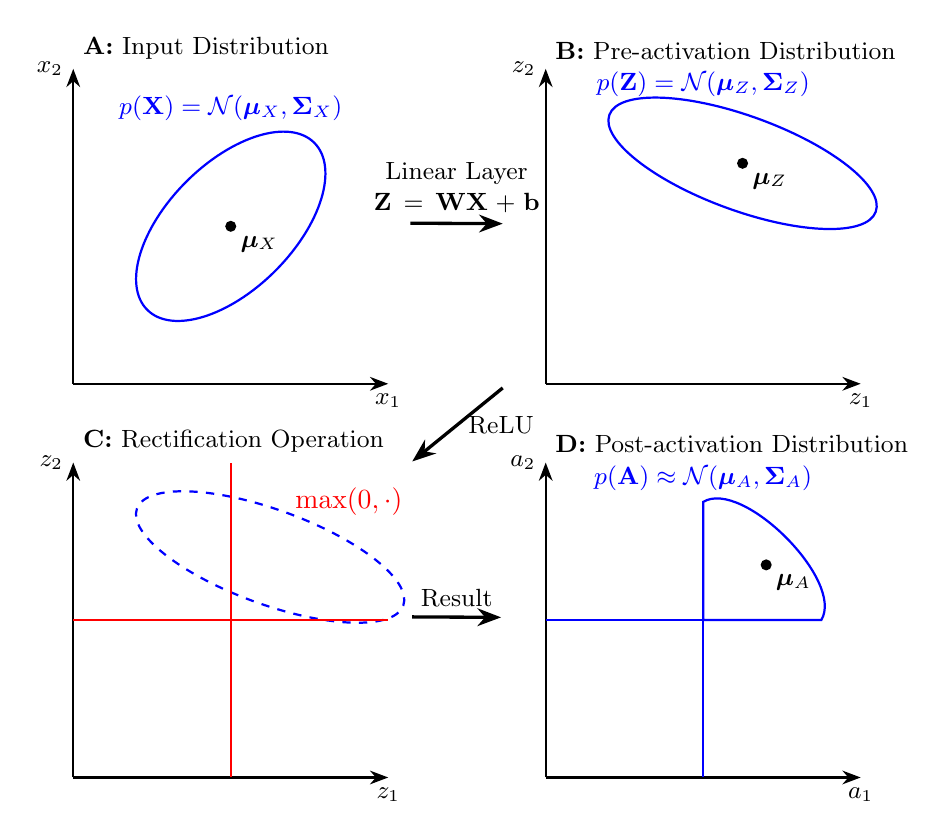
\begin{tikzpicture}[
        font=\sffamily,
        every node/.style={font=\small, align=center}
    ]
    % --- Panel A: Input Distribution ---
    \begin{scope}[local bounding box=panelA]
        \draw[-Stealth, thick] (-2,-2) -- (2,-2) node[below] {$x_1$};
        \draw[-Stealth, thick] (-2,-2) -- (-2,2) node[left] {$x_2$};
        \node[above right] at (-2,2) {\textbf{A:} Input Distribution};
        \draw[blue, thick, rotate around={45:(0,0)}] (0,0) ellipse (1.5cm and 0.8cm);
        \fill[black] (0,0) circle (2pt) node[below right] {$\boldsymbol{\mu}_X$};
        \node[blue] at (0, 1.5) {$p(\vect{X}) = \mathcal{N}(\boldsymbol{\mu}_X, \boldsymbol{\Sigma}_X)$};
    \end{scope}

    % --- Panel B: Linear Transformation ---
    \begin{scope}[local bounding box=panelB, xshift=6cm]
        \draw[-Stealth, thick] (-2,-2) -- (2,-2) node[below] {$z_1$};
        \draw[-Stealth, thick] (-2,-2) -- (-2,2) node[left] {$z_2$};
        \node[above right] at (-2,2) {\textbf{B:} Pre-activation Distribution};
        \draw[blue, thick, rotate around={-20:(0.5,0.8)}] (0.5,0.8) ellipse (1.8cm and 0.6cm);
        \fill[black] (0.5,0.8) circle (2pt) node[below right] {$\boldsymbol{\mu}_Z$};
        \node[blue] at (0, 1.8) {$p(\vect{Z}) = \mathcal{N}(\boldsymbol{\mu}_Z, \boldsymbol{\Sigma}_Z)$};
    \end{scope}

    % --- Panel C: Non-Linear Rectification ---
    \begin{scope}[local bounding box=panelC, yshift=-5cm]
        \draw[-Stealth, thick] (-2,-2) -- (2,-2) node[below] {$z_1$};
        \draw[-Stealth, thick] (-2,-2) -- (-2,2) node[left] {$z_2$};
        \node[above right] at (-2,2) {\textbf{C:} Rectification Operation};
        % Draw original ellipse for context
        \draw[blue, thick, dashed, rotate around={-20:(0.5,0.8)}] (0.5,0.8) ellipse (1.8cm and 0.6cm);
        % Draw axes for rectification
        \draw[red, thick] (-2,0) -- (2,0);
        \draw[red, thick] (0,-2) -- (0,2);
        \node[red, font=\bfseries] at (1.5, 1.5) {$\max(0, \cdot)$};
    \end{scope}

    % --- Panel D: Output Distribution (MODIFIED FOR ALIGNMENT) ---
    \begin{scope}[local bounding box=panelD, xshift=6cm, yshift=-5cm]
        \draw[-Stealth, thick] (-2,-2) -- (2,-2) node[below] {$a_1$};
        \draw[-Stealth, thick] (-2,-2) -- (-2,2) node[left] {$a_2$};
        \node[above right] at (-2,2) {\textbf{D:} Post-activation Distribution};
        % Draw an approximate shape for the rectified distribution, now centered
        \draw[blue, thick] (0,-2) -- (0,0) -- (-2,0); % Boundary axes
        \draw[blue, thick] (0,0) -- (0,1.5) .. controls (0.5,1.8) and (1.8,0.5) .. (1.5,0) -- (0,0);
        \fill[black] (0.8,0.7) circle (2pt) node[below right] {$\boldsymbol{\mu}_A$};
        \node[blue] at (0, 1.8) {$p(\vect{A}) \approx \mathcal{N}(\boldsymbol{\mu}_A, \boldsymbol{\Sigma}_A)$};
    \end{scope}

    % --- Arrows connecting panels ---
    \draw[-{Stealth[length=3mm]}, very thick] (panelA) -- (panelB) node[midway, above, text width=3cm] {Linear Layer \\ $\vect{Z} = \vect{W}\vect{X} + \vect{b}$};
    \draw[-{Stealth[length=3mm]}, very thick] (panelB) -- (panelC) node[midway, right] {ReLU};
    \draw[-{Stealth[length=3mm]}, very thick] (panelC) -- (panelD) node[midway, above] {Result};

    \end{tikzpicture}%
}

\ifdefined\ispartofbook
  % This part is intentionally left blank when included in the main book.
\else
  % This part is for standalone compilation of the image.
  \amplayerdiagram
  \end{document}
\fi
 % For standalone compilation
\fi

% This file defines the command for illustrating AMP through a single layer.
% It can be compiled standalone or included in a larger document.

\ifdefined\ispartofbook
\else
  % --- Standalone Compilation Preamble ---
  \documentclass[tikz, border=10pt]{standalone}
  \usepackage{tikz}
  \usetikzlibrary{arrows.meta, positioning}
  \usepackage{amsmath, amssymb} % Added for \vect command
  \newcommand{\vect}[1]{\mathbf{#1}} % Added for \vect command
  \begin{document}
\fi

% --- THE DIAGRAM COMMAND ---
\newcommand{\amplayerdiagram}{%
    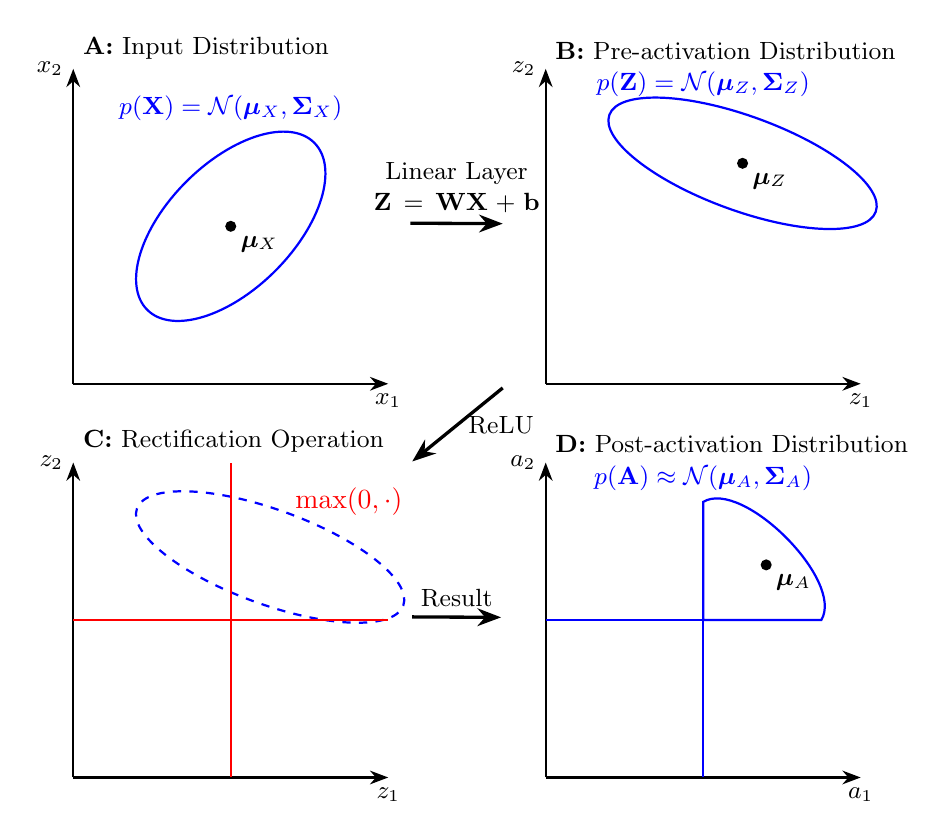
\begin{tikzpicture}[
        font=\sffamily,
        every node/.style={font=\small, align=center}
    ]
    % --- Panel A: Input Distribution ---
    \begin{scope}[local bounding box=panelA]
        \draw[-Stealth, thick] (-2,-2) -- (2,-2) node[below] {$x_1$};
        \draw[-Stealth, thick] (-2,-2) -- (-2,2) node[left] {$x_2$};
        \node[above right] at (-2,2) {\textbf{A:} Input Distribution};
        \draw[blue, thick, rotate around={45:(0,0)}] (0,0) ellipse (1.5cm and 0.8cm);
        \fill[black] (0,0) circle (2pt) node[below right] {$\boldsymbol{\mu}_X$};
        \node[blue] at (0, 1.5) {$p(\vect{X}) = \mathcal{N}(\boldsymbol{\mu}_X, \boldsymbol{\Sigma}_X)$};
    \end{scope}

    % --- Panel B: Linear Transformation ---
    \begin{scope}[local bounding box=panelB, xshift=6cm]
        \draw[-Stealth, thick] (-2,-2) -- (2,-2) node[below] {$z_1$};
        \draw[-Stealth, thick] (-2,-2) -- (-2,2) node[left] {$z_2$};
        \node[above right] at (-2,2) {\textbf{B:} Pre-activation Distribution};
        \draw[blue, thick, rotate around={-20:(0.5,0.8)}] (0.5,0.8) ellipse (1.8cm and 0.6cm);
        \fill[black] (0.5,0.8) circle (2pt) node[below right] {$\boldsymbol{\mu}_Z$};
        \node[blue] at (0, 1.8) {$p(\vect{Z}) = \mathcal{N}(\boldsymbol{\mu}_Z, \boldsymbol{\Sigma}_Z)$};
    \end{scope}

    % --- Panel C: Non-Linear Rectification ---
    \begin{scope}[local bounding box=panelC, yshift=-5cm]
        \draw[-Stealth, thick] (-2,-2) -- (2,-2) node[below] {$z_1$};
        \draw[-Stealth, thick] (-2,-2) -- (-2,2) node[left] {$z_2$};
        \node[above right] at (-2,2) {\textbf{C:} Rectification Operation};
        % Draw original ellipse for context
        \draw[blue, thick, dashed, rotate around={-20:(0.5,0.8)}] (0.5,0.8) ellipse (1.8cm and 0.6cm);
        % Draw axes for rectification
        \draw[red, thick] (-2,0) -- (2,0);
        \draw[red, thick] (0,-2) -- (0,2);
        \node[red, font=\bfseries] at (1.5, 1.5) {$\max(0, \cdot)$};
    \end{scope}

    % --- Panel D: Output Distribution (MODIFIED FOR ALIGNMENT) ---
    \begin{scope}[local bounding box=panelD, xshift=6cm, yshift=-5cm]
        \draw[-Stealth, thick] (-2,-2) -- (2,-2) node[below] {$a_1$};
        \draw[-Stealth, thick] (-2,-2) -- (-2,2) node[left] {$a_2$};
        \node[above right] at (-2,2) {\textbf{D:} Post-activation Distribution};
        % Draw an approximate shape for the rectified distribution, now centered
        \draw[blue, thick] (0,-2) -- (0,0) -- (-2,0); % Boundary axes
        \draw[blue, thick] (0,0) -- (0,1.5) .. controls (0.5,1.8) and (1.8,0.5) .. (1.5,0) -- (0,0);
        \fill[black] (0.8,0.7) circle (2pt) node[below right] {$\boldsymbol{\mu}_A$};
        \node[blue] at (0, 1.8) {$p(\vect{A}) \approx \mathcal{N}(\boldsymbol{\mu}_A, \boldsymbol{\Sigma}_A)$};
    \end{scope}

    % --- Arrows connecting panels ---
    \draw[-{Stealth[length=3mm]}, very thick] (panelA) -- (panelB) node[midway, above, text width=3cm] {Linear Layer \\ $\vect{Z} = \vect{W}\vect{X} + \vect{b}$};
    \draw[-{Stealth[length=3mm]}, very thick] (panelB) -- (panelC) node[midway, right] {ReLU};
    \draw[-{Stealth[length=3mm]}, very thick] (panelC) -- (panelD) node[midway, above] {Result};

    \end{tikzpicture}%
}

\ifdefined\ispartofbook
  % This part is intentionally left blank when included in the main book.
\else
  % This part is for standalone compilation of the image.
  \amplayerdiagram
  \end{document}
\fi
 % Include the AMP Layer diagram command file

\section{The Forward Pass on a Distribution}
\label{sec:forward_pass_distribution}

This subchapter provides the detailed mathematical derivations for the concepts introduced in Subchapter 7.1. We will explain how to analytically propagate the first two statistical moments—the mean vector and the covariance matrix—through a single, complete neural network layer. This process, known as Analytical Moment Propagation (AMP), involves two distinct steps: propagation through the layer's linear (affine) transformation and propagation through its non-linear activation function.

\subsection{Step 1: Propagation through the Linear Layer}
Let the input to a layer be an $N$-dimensional random vector $\vect{X}$ that follows a multivariate normal distribution, $\vect{X} \sim \mathcal{N}(\boldsymbol{\mu}_X, \boldsymbol{\Sigma}_X)$. The first operation in a standard dense layer is the affine transformation to compute the pre-activation vector $\vect{Z}$:
\begin{equation}
    \vect{Z} = \vect{W}\vect{X} + \vect{b}
\end{equation}
where $\vect{W}$ is the weight matrix and $\vect{b}$ is the bias vector.

Because the multivariate normal distribution is closed under affine transformations, the resulting pre-activation vector $\vect{Z}$ is also exactly normally distributed. We can find its mean and covariance using the standard rules for linear transformations of random vectors:
\begin{itemize}
    \item \textbf{The new mean vector, $\boldsymbol{\mu}_Z$,} is found by applying the transformation to the original mean:
    \begin{equation}
        \boldsymbol{\mu}_Z = \E[\vect{W}\vect{X} + \vect{b}] = \vect{W}\E[\vect{X}] + \vect{b} = \vect{W}\boldsymbol{\mu}_X + \vect{b}
    \end{equation}
    \item \textbf{The new covariance matrix, $\boldsymbol{\Sigma}_Z$,} is found by transforming the original covariance:
    \begin{equation}
        \boldsymbol{\Sigma}_Z = \text{Cov}(\vect{W}\vect{X} + \vect{b}) = \vect{W}\text{Cov}(\vect{X})\vect{W}^T = \vect{W}\boldsymbol{\Sigma}_X\vect{W}^T
    \end{equation}
\end{itemize}
This first step is analytically exact and straightforward. It transforms the input Gaussian distribution into a new Gaussian distribution that has been rotated, scaled, and shifted in the vector space.

\subsection{Step 2: Propagation through the Non-Linear (ReLU) Layer}
The second step presents the core analytical challenge. The pre-activation vector $\vect{Z} \sim \mathcal{N}(\boldsymbol{\mu}_Z, \boldsymbol{\Sigma}_Z)$ is passed through the element-wise ReLU activation function to produce the post-activation vector $\vect{A}$:
\begin{equation}
    \vect{A} = \max(\vect{0}, \vect{Z})
\end{equation}
The resulting distribution, $p(\vect{A})$, is a Rectified Multivariate Normal (RMVN) distribution, which is no longer Gaussian. As discussed in Chapter \ref{chap:multivariate_stats}, its moments are analytically intractable for high dimensions. Therefore, AMP proceeds by computing the exact first two moments of this non-Gaussian distribution.

The mean and variance of each component $A_i$ can be computed independently using the univariate rectified Gaussian formulas from Chapter 1. Let $(\mu_Z)_i$ be the $i$-th component of $\boldsymbol{\mu}_Z$ and $(\sigma_Z)_i = \sqrt{(\boldsymbol{\Sigma}_Z)_{ii}}$ be its standard deviation.
\begin{itemize}
    \item \textbf{The new mean vector, $\boldsymbol{\mu}_A$}, has components given by:
    \begin{equation}
        (\boldsymbol{\mu}_A)_i = \E[A_i] = (\mu_Z)_i \Phi\left(\frac{(\mu_Z)_i}{(\sigma_Z)_i}\right) + (\sigma_Z)_i \phi\left(\frac{(\mu_Z)_i}{(\sigma_Z)_i}\right)
    \end{equation}
    \item \textbf{The new covariance matrix, $\boldsymbol{\Sigma}_A$}, is more complex. The diagonal elements (the variances) can be computed element-wise:
    \begin{equation}
        (\boldsymbol{\Sigma}_A)_{ii} = \text{Var}(A_i) = \E[A_i^2] - (\E[A_i])^2
    \end{equation}
    However, the off-diagonal elements, $\text{Cov}(A_i, A_j)$, depend on the correlation between the pre-activations $Z_i$ and $Z_j$ and require the evaluation of high-dimensional integrals. State-of-the-art AMP frameworks use sophisticated analytical theorems or accurate approximations to compute this full covariance matrix \cite{Wright2024AnalyticCovariance, FreyHinton1999Transformations}.
\end{itemize}

\begin{figure}[h!]
    \centering
    \scalebox{0.7}{\amplayerdiagram}
    \caption{Analytical Moment Propagation through a Single Layer. (A) The input is modeled as a Gaussian distribution. (B) The linear layer rotates, scales, and shifts the distribution. (C) The ReLU activation rectifies the distribution, projecting it onto the non-negative quadrant. (D) The resulting post-activation distribution is non-Gaussian, but its first two moments can be calculated.}
    \label{fig:amp_layer}
\end{figure}

The figure above provides a visual summary of this entire process. It illustrates how a simple, symmetric input distribution is warped by the layer's operations into a complex, non-Gaussian output distribution. The core of forward AMP is the set of mathematical rules that allow us to calculate the parameters of this output distribution without ever needing to sample individual data points.

\ifdefined\ispartofbook
\else
  \end{document}
\fi
